\newpage
\section{Durchführung}\label{sec:durchfuehrung}
In diesem Kapitel werden die Szenarien im Detail beschrieben,
sowie deren Paketmittschnitte analysiert.
Die Analyse beschränkt sich hierbei auf Nachrichten der Geräte untereinander
und auf mit dem Szenario zusammenhängende Pakete an andere Geräte/Server im Internet.

\subsection{Jeweils eine Minute ohne Aktionen bei ein- und ausgeschalteter Konsole}\label{sec:durchfuehrung-aus}
Ziel dieses Szenarios ist es die Kommunikation zu ermitteln,
welche zwischen den Geräten stattfindet,
ohne dass durch den Benutzer ein Befehl erteilt wurde.
Es zeigt sich, dass die Geräte auch im Ruhezustand rege miteinander Informationen austauschen.

\paragraph{Home Assistant und Playstation 4}
Der Home Assistant wurde so konfiguriert,
dass er regelmäßig den Status der \ac{ps4} überprüft.
Dies geschieht über ein UDP-Paket,
welches an Port \texttt{987} der Broadcast-Adresse \texttt{255.255.255.255} gesendet wird.
Über das Senden an die Broadcast-Adresse wird erreicht,
dass der Router das Paket an alle lokalen Geräte verteilt.
\texttt{987} wiederum ist der Port, über welchen die Spielekonsole UDP-Pakete annimmt.

Der Inhalt des Pakets (siehe \autoref{lst:ps4-wakeup_search}) besteht aus dem Kommando \texttt{SRCH},
der HTTP-Version und einer \texttt{device-discovery-protocol-version}.
Vermutlich steht das Kürzel \texttt{SRCH} für \enquote{Search}.
Mit disem Paket werden keine Aktionen ausgeführt,
sondern nur Systeminformationen angefordert.

\lstinputlisting[
    caption=Daten eines SRCH-Paketes,
    label=lst:ps4-wakeup_search
]{ps4_search.udp}

\newpage

Auf dieses Paket antwortet die \ac{ps4} ebenfalls mit einem UDP-Paket,
welches verschiedenen Geräteinformationen enthält.

Vergleicht man die Antworten der eingeschalteten (\autoref{lst:ps4-wakeup_search_respOn})
und ausgeschalteten (\autoref{lst:ps4-wakeup_search_respOff}) \ac{ps4} miteinander,
so ist festzustellen,
dass sich die jeweiligen Antworten lediglich im Statuscode der ersten Zeile unterscheiden.
\texttt{200 Ok} gibt an, dass die Playstation 4 eingeschaltet und \texttt{620 Server Standby},
dass die ausgeschaltet (bzw. im Standby-Modus) ist.

\lstinputlisting[
    caption=Antwort auf SRCH-Paket (Eingeschaltet),
    label=lst:ps4-wakeup_search_respOn
]{ps4_search_respOn.udp}

\lstinputlisting[
    caption=Antwort auf SRCH-Paket (Ausgeschaltet),
    label=lst:ps4-wakeup_search_respOff
]{ps4_search_respOff.udp}

\newpage
\paragraph{Home Assistant und Harmony Hub}
Um ebenfalls regelmäßig den aktuellen Status der Spielekonsole zu erfahren,
erfragt der Harmony Hub diese Information beim Home Assistant über die emulierte \textit{Hue Bridge}.
Dies geschieht in Form eines HTTP-GET-Requests,
welcher über eine für diesen Zweck errichte TCP-Verbindung erfolgt.
Der Request erfolgt an die URL \nolinkurl{192.168.178.45:8300/api/12345678901234567890/lights}.

Über den Port \texttt{8300} wird die emulierte \textit{Hue Bridge} erreicht,
welche über den angegebenen Pfad Informationen über alle eingerichteten \enquote{Leuchten}
(darunter auch der Schalter zur Kontrolle der \ac{ps4}) bereitstellt.

Als Antwort liefert Home Assistant mehrere Objekte im JSON-Format.
Der Teil der Antwort welcher den Schalter,
ist in \autoref{lst:ps4_get} dargestellt.
Hervorzuheben sind hier folgende Felder:
\lstinline[language=json]{"name"} enthält den nutzerfreundlichen Namen,
welcher in der Konfiguration angegeben wurde.
\lstinline[language=json]{"uniqueid"} enthält die
in der Konfiguration gesetzte ID mit dem zusätzlichen Präfix \lstinline[language=json]{"switch"}.
Das Feld \lstinline[language=json]{"on"} gibt an, ob die Leuchte (und damit die Spielekonsole) gerade eingeschaltet ist.
In diesem Fall ist sie ausgeschaltet, weshalb dieser Wert \lstinline[language=json]{false} ist.

\lstinputlisting[
    caption=Nutzdaten GET-Response (gekürzt),
    label=lst:ps4_get,
    language=json
]{ps4_get.json}

\newpage

\subsection{Ein- und Ausschalten über Home Assistant}\label{sec:durchfuehrung-hassbian}
\hyphenation{Web-ober-fläche}
Der Home Assistant bietet zur Steuerung der konfigurierten Geräte eine Weboberfläche.
In \autoref{fig:hass-ui} ist der Schalter hervorgehoben, welcher für das Ein- und Ausschalten der Playstation 4 genutzt wird.

\begin{figure}[h!]
    \centering
    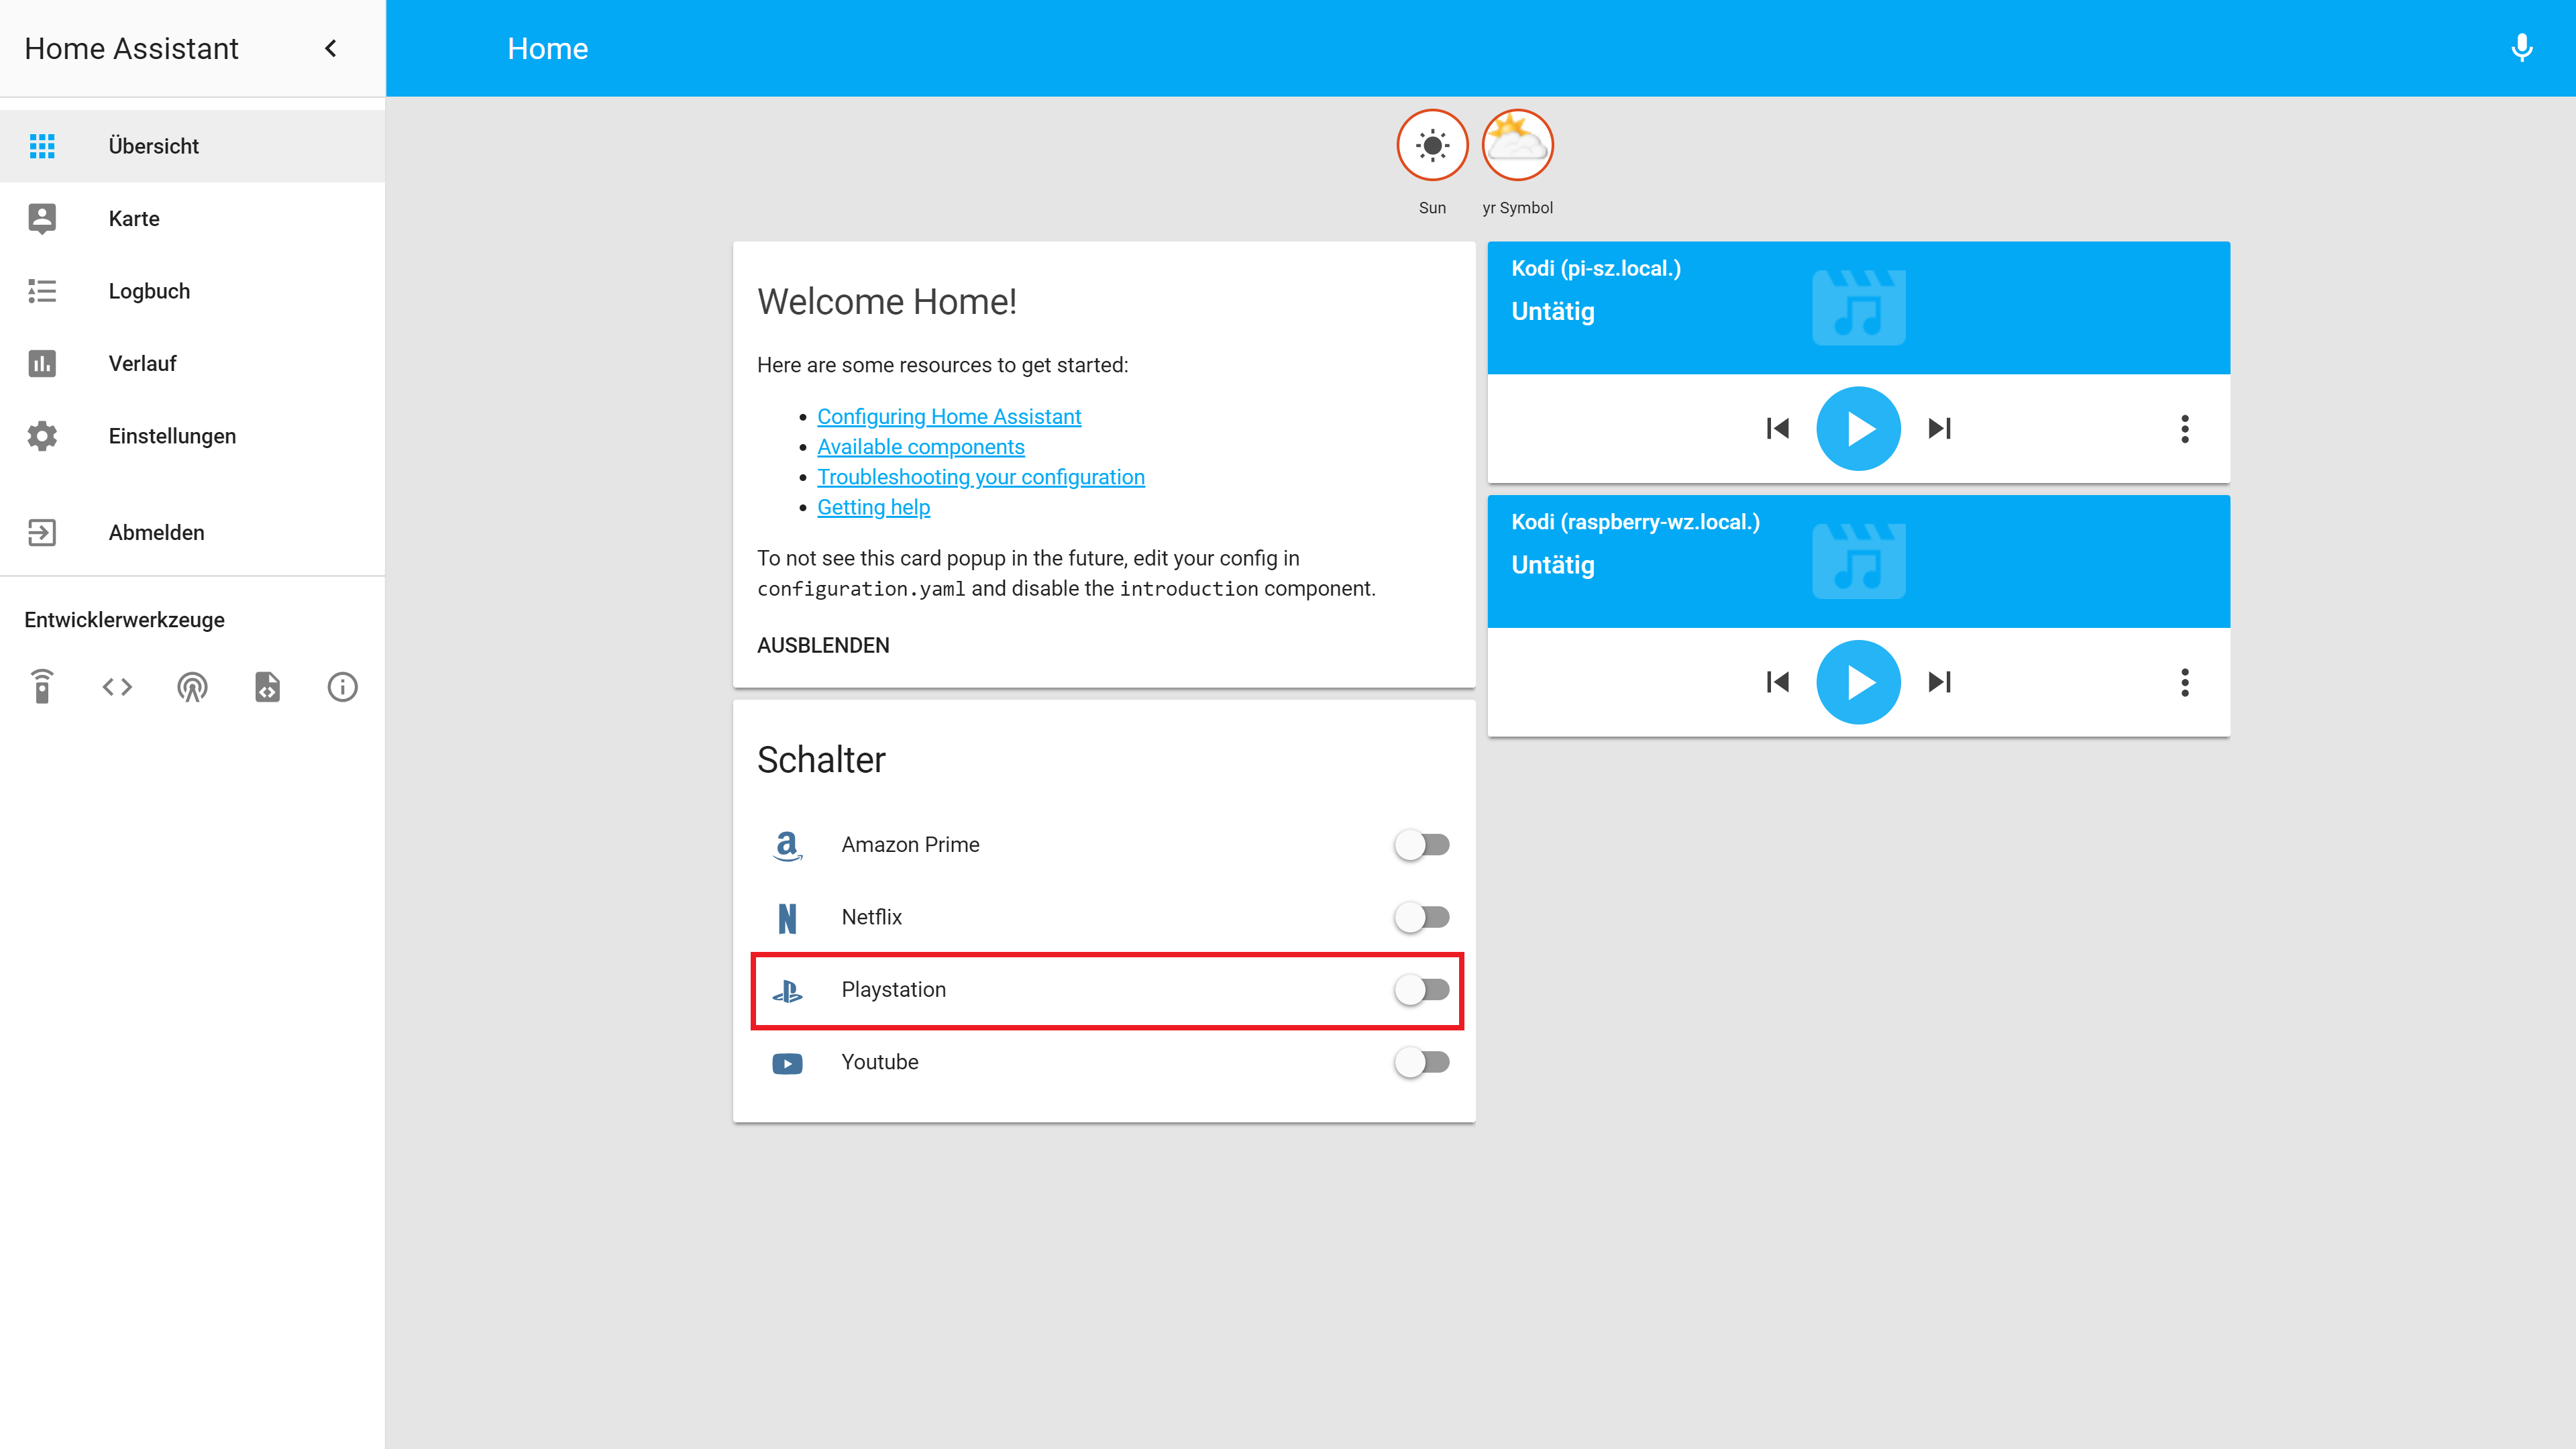
\includegraphics[width=\textwidth]{hass_ui}
    \caption{Weboberfläche des Home Assistant}\label{fig:hass-ui}
\end{figure}

Sowohl beim Ein- als auch beim Ausschalten werden zusätzlich zu dem bereits bekannten \texttt{SRCH}-Paket
zwei weitere Arten von UDP-Paketen gesendet.
Das eine enthält den Befehl \texttt{WAKEUP} (\autoref{lst:ps4-wakeup}),
das andere den Befehl \texttt{LAUNCH} (\autoref{lst:ps4-launch}).

\lstinputlisting[
    caption=Daten eines WAKEUP-Paketes,
    label=lst:ps4-wakeup
]{ps4_wakeup.udp}


Das Feld \texttt{user-credential} (in den Listings gekürzt) ist hierbei immer gleich.
Der darin enthaltene Wert wurde beim initialen Verbindungsaufbau automatisch ermittelt.
Es werden zwei \texttt{WAKEUP}-Pakete und ein \texttt{LAUNCH}-Paket gesendet,
um zu prüfen, ob die \ac{ps4} bereit ist eine Verbindung anzunehmen.

\lstinputlisting[
    caption=Daten eines LAUNCH-Paketes,
    label=lst:ps4-launch
]{ps4_launch.udp}

Der eigentliche Befehl wird in einer, auf die UDP-Pakete folgenden, TCP-Verbindung ausgeführt.
Zwar ist diese Verbindung nicht mit TLS verschlüsselt,
die Daten können dennoch nicht ausgelesen werden.

Der Grund hierfür ist im Quellcode des \textit{ps4-waker} ersichtlich \cite{ps4waker31:online}\cite{ps4waker93:online}:
Die Daten werden dort vor dem Senden (und damit auf Anwendungsebene) verschlüsselt.
Ein weiterer Blick in den Quellcode zeigt den Aufbau der TCP-Pakete.
Der Paket-Typ (auf Anwendungsebene) wird durch eine Ganzzahl angegeben.
Zusätzlich werden je nach Anwendungsfall ASCII Zeichen oder Ganzzahlen übertragen,
um die gewünschten Befehle auszuführen.
Das Paket eines Standby-Befehls wird beispielsweise wie in \autoref{lst:ps4-standby} erstellt und gesendet (aus \cite{ps4waker31:online}).

\lstinputlisting[
    caption=Erstellen und Senden eines Standby-Befehls,
    label=lst:ps4-standby,
    firstnumber=273
]{ps4_standby.js}

Durch diese Funktionsaufrufe wird ein TCP-Paket der Länge 8 Bytes erstellt,
mit der Zahl 26 gefüllt,
verschlüsselt und gesendet.

\newpage

\subsection{Ein- und Ausschalten über \textit{Harmony Hub}}\label{sec:durchfuehrung-harmony}
Im Harmony Hub ist zur Nutzung der Playstation 4 eine Aktion namens \enquote{Spielen} konfiguriert.
Zusätzlich zur Spielekonsole wird in dieser Aktion auch der Fernseher ein- bzw. ausgeschaltet.

Zum Einschalten wird der durch den Home Assistant bereitgestellte Schalter genutzt.
Dieser wird über die emulierte \textit{Hue Bridge} durch den Harmony Hub aktiviert.

Ist die \ac{ps4} eingeschaltet, so kann der Hub eine Bluetooth-Verbindung aufbauen.
Daher ist es zum Ausschalten nicht nötig den Home Assistant zu nutzen.
Der Hub schaltet die Konsole direkt über die Bluetooth-Verbindung aus,
sobald die Aktion \enquote{Spielen} beendet wird.

\subsubsection{Einschalten}
Der Paketmitschnitt enthält mehrere TCP-Verbindungen.
An der Kommunikation sind der Harmony Hub, der \textit{Home Assistant} und die \ac{ps4} beteiligt.
Zusätzlich frägt der Harmony Hub per DNS die IP-Adresse von \nolinkurl{home.myharmony.com} an.
Als Antwort wird auf den Server mit der URL \nolinkurl{home-myharmony.us-east-1.elasticbeanstalk.com} verwiesen.
Die TCP-Verbindung zwischen Harmony Hub und Webserver ist durch TLS verschlüsselt.

Der \textit{Home Assistant} und die \ac{ps4} kommunizieren, wie bereits im vorigen Abschnitt untersucht, mittels TCP und UDP.
Der Harmony Hub kommuniziert mit \textit{Home Assistant} über HTTP.

Der Ablauf der Kommunikation wird in \autoref{fig:ps-ein-harmony} vereinfacht dargestellt.
Bei HTTP-Verbindungen wird lediglich das HTTP-Paket gezeigt,
der TCP-Rahmen mit Verbindungsaufbau und -abbau wird nicht abgebildet.
Außerdem fehlen in der Abbildung die UDP-Pakete,
welche vom \textit{Home Assistant} genutzt werden,
um den Status der \ac{ps4} zu erfragen.

\begin{figure}
    \centering
    \resizebox{\textwidth}{!}{
        \input{assets/uml/ps-ein-harmony.latex}
    }
    \caption{Kommunikation beim Einschalten}
    \label{fig:ps-ein-harmony}
\end{figure}

\newpage



\paragraph{Harmony Hub und Webserver}
Die Verbindungen sind verschlüsselt.
Daher können zum genauen Inhalt und Zweck keine Aussagen getroffen werden.
Vermutlich dienen sie dazu, Informationen über die gestartete Aktion zu übergeben.

Bei genauerer Betrachtung eines Paketes, welches vom Harmony Hub an den Webserver gesendet wird,
sind verschiedene Besonderheiten zu erkennen:

\begin{figure}[h!]
    \centering
    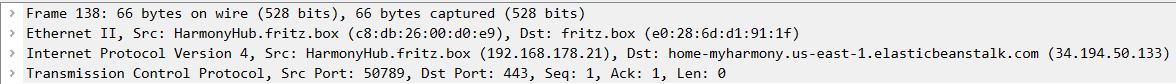
\includegraphics[width=\textwidth]{internet-paket}
    \caption{Paket von Harmony Hub an Webserver}\label{fig:internet-paket}
\end{figure}


\autoref{fig:internet-paket} zeigt die verschiedenen Protokoll-Header, welche ineinander verschachtelt sind.
Die oberste Zeile (\textit{Frame}) steht für das gesamte Paket.

In der zweiten Zeile steht die äußerste Paket-Schicht \textit{Ethernet II}.
Deren Quelladresse ist die MAC-Adresse des Harmony Hub.
Als Zieladresse ist jedoch nicht die MAC-Adresse des Webservers,
sondern die der FRITZ!Box angegeben.
Dies liegt daran, dass Ethernet lediglich zur Kommunikation im lokalen Netz verwendet wird.
Das Paket wird per Ethernet an die FRITZ!Box gesendet.
Dort wird die \enquote{Ethernet-Nutzlast} (das IP-Paket inklusive TCP; Zeile 3) entpackt und über \textit{IPv4} an das eigentliche Ziel weitergeleitet.
Dessen Adresse ist als Zieladresse im IP-Header angegeben.

Da die Verbindung verschlüsselt ist, lassen sich aus den übertragenen Daten keine Informationen gewinnen.
Der Zielport des TCP-Headers in der letzen Zeile liefert jedoch einen Hinweis auf die Methode der Übertragung.
Der Port \textit{443} wird standardmäßig für \textit{HTTPS}-Verbindungen genutzt.
Daraus und aus der Tatsache, dass die Verbindung mittels TLS verschlüsselt ist,
lässt sich mit hoher Wahrscheinlichkeit schließen, dass tatsächlich \textit{HTTPS} genutzt wird.

\paragraph{Home Assistant und Playstation 4}
Ziwschen diesen Geräten läuft die Kommunikation nach den gleichen Schema ab,
wie es bereits im vorigen Abschnitt betrachtet wurde.

\paragraph{Home Assistant und Harmony Hub}
Auch während des Einschaltens werden HTTP-GET-Requests (siehe Kapitel \ref{sec:durchfuehrung-aus}) genutzt,
um vom Harmony Hub aus den Status der \ac{ps4} zu erfragen.

Zusätzlich wird ein HTTP-PUT-Request gesendet, wodurch der Befehl das Gerät einzuschalten übermittelt wird.
Dieser Request wird an die Adresse \nolinkurl{http://192.168.178.45:8300/api/12345678901234567890/lights/1/state} gesendet.

Die angegebene IP-Adresse ist die des Raspberry PI, welcher an Port 8300 Befehle an die emulierte \textit{Hue Bridge} des \textit{Home Assistant} entgegennimmt.
\texttt{/api/\\12345678901234567890/lights/1} wählt das zu kontrollierende Gerät aus.
Wie in Kapitel \ref{sec:aufbau-hassbian} beschrieben, werden die Geräte nach außen hin als Lichter (engl. Lights) präsentiert.
Als Nutzdaten enthält das Paket die in \autoref{lst:ps4_on-request} gezeigten Daten im JSON-Format.

\lstinputlisting[
    caption=Nutzdaten PUT-Request,
    label=lst:ps4_on-request,
    language=json
]{ps4_on-request.json}

Für diesen Anwendungsfall ist einzig der Wert \lstinline[language=json]{"on": true} von Relevanz.
Mit dem Wert \lstinline[language=json]{"x,y"} könnte bei echten Lampen die Farbe
und mit dem Wert \lstinline[language=json]{"bri"} die Helligkeit gesteuert werden \cite{Coreconc26:online}.


Die Antwort auf den PUT-Request enthält ebenfalls Daten im JSON-Format,
um den Erfolg des Befehls mitzuteilen (siehe \autoref{lst:ps4_on-response}).
\lstinputlisting[
    caption=Nutzdaten PUT-Request,
    label=lst:ps4_on-response,
    language=json
]{ps4_on-response.json}

\newpage
\subsubsection{Ausschalten}
Da zum Ausschalten der \ac{ps4} der \textit{Home Assistant} nicht genutzt wird,
fällt die Netzwerkkommunikation hier deutlich sparsamer aus.

Wieder kommuniziert der Harmony Hub verschlüsselt mit \nolinkurl{home.myharmony.com}.
Außerdem wird der Status der Konsole vom Harmony Hub beim \textit{Home Assistant} über die bereits bekannten GET-Requests erfragt.
Der \textit{Home Assistant} erhält den Status der Konsole wiederum durch die SRCH-Pakete.

\begin{figure}[ht!]
    \centering
    \resizebox{\textwidth}{!}{
        \input{assets/uml/ps-aus-harmony.latex}
    }
    \caption{Kommunikation beim Ausschalten}
    \label{fig:ps-aus-harmony}
\end{figure}

In \autoref{fig:ps-aus-harmony} ist der Ablauf beim Ausschalten dargestellt.
Im Gegensatz zum vorigen Ablaufdiagramm sind hier die SRCH-Pakete abgebildet.
Außerdem ist zu den Antworten auf die Statusanfrage notiert,
ob die \ac{ps4} zu diesem Zeitpunkt ein- oder ausgeschaltet ist.

Aus dem Ablauf ist zu erkennen,
dass die Konsole zwischen dem zweiten GET- und dem zweiten SRCH-Paket ausgeschaltet wurde.
Da dies über einen anderen Kanal (Bluetooth) geschieht,
finden sich im Paketmittschnitt zum Ausschalten selbst keine Nachrichten.